%% +++++++++++++++++++++++++++++++++
%% Setzen von scrreprt
%% +++++++++++++++++++++++++++++++++
\documentclass[
11pt,
titlepage,
a4paper,
abstracton,
twoside,
openright,
chapterprefix,
noappendixprefix,
headsepline,
footsepline,
cleardoubleplain,
bibtotoc,
liststotoc,
pointlessnumbers,
article
]{scrreprt}

%% +++++++++++++++++++++++++++++++++
%% Einbinden von Paketen
%% +++++++++++++++++++++++++++++++++
\usepackage{istitle}
\usepackage{geometry}
\usepackage[utf8]{inputenc} 
\usepackage[T1]{fontenc}
\usepackage{ae,aecompl}
\usepackage{amsmath}
\usepackage{amsthm}
\usepackage{amscd}
\usepackage{amsfonts}
\usepackage{amssymb}
\usepackage{listings}
\usepackage{xcolor}
\usepackage[english]{babel}
\usepackage{graphicx}
\usepackage{url}
\usepackage[automark]{scrlayer-scrpage}
\usepackage{natbib}
\usepackage{bbm}
\usepackage{array}
\usepackage{booktabs}
\usepackage{threeparttable}
\usepackage{pifont}
\usepackage{placeins}
\usepackage[font=small,labelfont=bf,labelsep=colon]{caption}
\usepackage{fancyhdr}
\usepackage[
backend=biber,
style=ieee,
]{biblatex}
\addbibresource{literatur.bib}
% Settings for generating the PDF
% See https://www.tug.org/applications/hyperref/manual.html

\usepackage{hyperref}

\hypersetup{
	pdfinfo={ 
    		Title={Diplomarbeit},
		Creator={TeX},
		Producer={pdfTeX 0.15a},
		Author={},
		CreationDate={D:20091004000000},
		ModDate={D:20130331000000},
		Subject={Master thesis},
		Keywords={}
	},
	pdfpagelayout=TwoColumnRight,
	pdfdisplaydoctitle=true
}



%% Settings for generating the PDF
% See https://www.tug.org/applications/hyperref/manual.html


\hypersetup{
}


 % Links klickbar, vom PDF-Viewer hervorgehoben
%% Settings for generating the PDF
% See https://www.tug.org/applications/hyperref/manual.html


\hypersetup{
	colorlinks, % colored links
	linkcolor=blue,
	filecolor=darkgreen,
	urlcolor=red,
	citecolor=green,
	hypertexnames=false,
}
 % Links klickbar, farbig hervorgehoben
% Settings for generating the PDF
% See https://www.tug.org/applications/hyperref/manual.html


\hypersetup{
	hidelinks=true % for hiding links altogether
}


 % Links klickbar, aber nicht hervorgehoben
\providecommand{\keywords}[1]
{
  \small	
  \textbf{\textit{Keywords:}} #1
}



%% +++++++++++++++++++++++++++++++++
%% Header
%% +++++++++++++++++++++++++++++++++

% Seitengeometrie
\geometry{a4paper,outer=38mm,inner=26mm,top=40mm,bottom=50mm}

% Definition von arg max
\DeclareMathOperator*{\argmax}{arg\,max}

% Definition von Sternchen
\newcommand{\sig}{\ding{73}}
\newcommand{\ssig}{\ding{72}}

% Definition von Häkchen und Kreuzchen
\newcommand{\h}{\ding{51}}
\newcommand{\x}{\ding{55}}

% Farben definieren
\definecolor{lightgrey}{rgb}{0.99,0.99,0.99}
\definecolor{colKeys}{rgb}{0,0,1}
\definecolor{colIdentifier}{rgb}{0,0,0}
\definecolor{colComments}{rgb}{1,0,0}
\definecolor{colString}{rgb}{0,0.5,0}

\definecolor{darkred}{rgb}{0.5,0,0}
\definecolor{darkgreen}{rgb}{0,0.5,0}
\definecolor{darkblue}{rgb}{0,0,0.5}
\definecolor{green}{rgb}{0,0.7,0}
\definecolor{blue}{rgb}{0,0,0.7}
\definecolor{red}{rgb}{0.7,0,0}
\definecolor{black}{rgb}{0,0,0}

% Quellcode
\lstloadlanguages{XML} 
\lstset{
  language = Haskell,
  basicstyle={\fontsize{10pt}{12pt}\ttfamily},
  columns=flexible,
  keepspaces=true,
  showstringspaces=false,
  identifierstyle=\color[rgb]{0.1,0.1,0.1},
  keywordstyle=\color{blue},
  commentstyle=\color[rgb]{0,0.3,0},
  frame=tb,                      
}

% Kopf- und Fußzeilen
\pagestyle{fancy}
\fancypagestyle{preContent}{
    \fancyhead{}
    \renewcommand\headrulewidth{0pt}
    \fancyfoot[C]{\thepage}
}

% Absätze
\setlength{\parindent}{0pt}
\setlength{\parskip}{2ex}

\def\topfraction{1.0} 
\def\bottomfraction{1.0} 
\def\textfraction{0.0}

\renewcommand*{\partpagestyle}{empty}

% Überschrift des Abstracts
\addto\captionsngerman{\renewcommand*\abstractname{Kurzzusammenfassung}}
% Überschrift des Verzeichnisses der Listings
\addto\captionsngerman{\renewcommand*\lstlistlistingname{Auflistungsverzeichnis}}
% Name von Listings
\addto\captionsngerman{\renewcommand*\lstlistingname{Auflistung}}


%% +++++++++++++++++++++++++++++++++
%% Start des Dokuments
%% +++++++++++++++++++++++++++++++++
\begin{document}

% Titelseite
\title{Structural checking and generation of mathematical representations of UML state diagrams}
\author{Le Zhang}
\tutor{Prof. Dr. Janis Voigtländer}
{M. Sc. Marcellus Siegburg}
\thesistype{Bachelor Thesis}

\logo{Bilder/logo_uni.png}
\timeperiod{September 2021}{December 2021}
\pagenumbering{alph}
\maketitle

% Kurzzusammenfassung (Abstract)
\setcounter{page}{2}
\begin{abstract}
\thispagestyle{plain}
UML state machine \cite{harel_naamad_1996} ,also known as UML statechart, is used to describe and the design of complex discrete-events systems \cite{harel_1987,harel_naamad_1996}.
Understanding state machine diagrams is essential for object-oriented software design.
So teaching this knowledge is an important part of many computer science modules.
For the purpose of E-learning,  we want to design a tool in Haskell for the automatic generation of UML state machine tasks.
The paper thoroughly discusses testing properties for our existing state diagram drawing tool in Haskell \cite{jun_hao_tan} and how to generate random test cases satisfying these criteria.
Firstly, we discuss in detail the essential constraints and invariants for a state diagram and how this model-checking tool is realized in Haskell. 
Then we introduce the random diagram generator. 
Finally, randomly generated expressions are fed to the program to discover errors with our software and visualize the diagram.

\keywords{ UML state diagram, QuickCheck, E-Learning, Haskell, Fuzzing}

\end{abstract}

% Inhaltsverzeichnis
\pagestyle{preContent}
\pagenumbering{Roman}
\setcounter{tocdepth}{2}
\tableofcontents

% Text
\cleardoublepage
\pagestyle{preContent}
\pagenumbering{arabic}
\sloppy
\chapter{Introduction}
\section{Motivation}
UML state machine is an effective tool for specification and designing complex systems. 
Our primary focus is to present an automatic generator of UML state diagrams in Haskell for university E-learnings.
Hence, we have done some limitations on the model, like the depth of a diagram will be no more than 4. 
These customizations could be modified by changing the corresponding value in the \verb| randomSD| (details see section \ref{sec:generator}).

The existing data type for the UML state diagram in the previous work \cite{jun_hao_tan} does not prevent abnormal or non-sense expressions, nor does the current model-checking functions rule them out. 
Those illegal expressions may also cause execution crashes.
Therefore, we need to define data structure properties and semantics more thoroughly for meaningful diagrams, then implement them in Haskell functions to automatically check violations in expressions.
Moreover, when we implement the generator, if the produced random data could pass all the checkers, we can say that it will generate expressions that the drawing tool will not fail and fit the actual UML state diagram.


\section{Outline}
The rest of the paper is organized as follows: "\nameref{chap:background}" section presents background knowledge on the UML state diagram, our existing UML state diagram drawing tool and checkers, and the technique for random testing, QuickCheck, which is fundamental for the automatic generator.
In the "\nameref{chap:implementation}" section, we illustrate the main constraints for model checking and how we realized the testing properties checking tool, the random generator in Haskell.
 "\nameref{chap:evaluation}" section gives an analysis of fuzzing test, coverage of our test suites, shows results of our random state diagram generator, and discusses the errors found during testing.
In the "\nameref{chap:Related and Future Work}" section, we summarize the possible aspects we might improve and focus on in the future and conclude our paper.
\chapter{Background}
\label{chap:background}

\section{ UML State Diagram}
The Unified Modeling Language\cite{miles_hamilton_2008} (UML) is a standard modeling language for system and software designing and specification. 
It isn't easy to develop a large-scale system.
Too many details can be misinterpreted or forgotten in the development process without some aids. 
Modeling allows us to have a clear vision of the system and capture and communicate with others the essential part of the system. 
So it is quite effective to model a system using the modeling language. 

UML has many types of diagrams. 
Some are static structural, and the rest are dynamic and describe the system's behaviour\cite{UML}. 
The figure shows the hierarchical classification of UML diagrams. 
The version of UML is still being updated and improved today. 
Our concern will only be on the UML state machine diagram, which is dynamic and shows the relations between internal states.
\begin{figure}[ht]
    \centering
    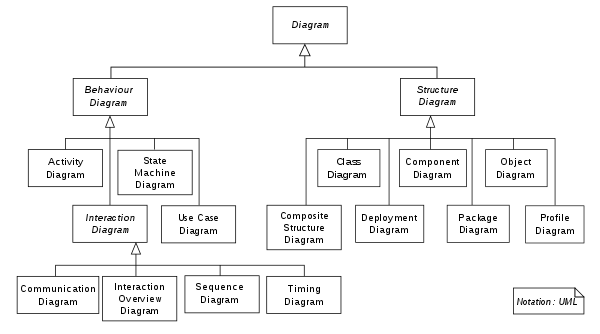
\includegraphics[scale=0.6]{Bilder/UMLOverview.png}
    \caption{The hierarchical classification of UML diagrams\cite{UML}}
    \label{fig:classification}
\end{figure}

UML state machine diagram is also informally called state diagram and in the past is referred to statechart \cite{harel_1987}.
We will illustrate some necessary notations of state diagrams in our current work.

\textbf{State} A state is represented by a rectangle with the state's name in the center. 
If the transition has an effect associated with it, we can also put the effect on the states. 
The diagram represents a state with entry action and exit action.
Actions that occur on events or always occur can also be defined as internal behaviour\cite{state_machine_diagram}.


\begin{figure}[htbp]
\begin{minipage}[t]{0.4\textwidth}
\centering
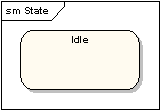
\includegraphics[width=4cm]{Bilder/sm1.png}
\caption{States\cite{state_machine_diagram}}
\end{minipage}
\begin{minipage}[t]{0.4\textwidth}
\centering
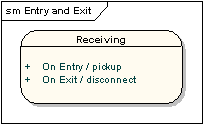
\includegraphics[width=5cm]{Bilder/sm2.png}
\caption{With internal behaviour\cite{state_machine_diagram}}
\end{minipage}
\end{figure}

\textbf{Initial and Final States}
A small filled black circle shows the initial state. 
A circle with a dot inside denotes the final state. 
The initial state should only have outgoing edges.
In contrast, the final state should only have ingoing edges.
\begin{figure}[ht]
    \centering
    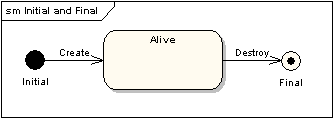
\includegraphics[scale=0.55]{Bilder/sm3.png}
    \caption{Initial and Final States\cite{state_machine_diagram}}
    \label{fig:picture4}
\end{figure}

\textbf{History States}
There are two types of history, shallow and deep.
A history state is used to remember the last exited state when interrupted and can be visited after recovery.
\begin{figure}[htbp]
\begin{minipage}[t]{0.4\textwidth}
\centering

\includegraphics[width=1cm]{Bilder/shallow.png}
\caption{Shallow history}
\end{minipage}
\begin{minipage}[t]{0.4\textwidth}
\centering

\includegraphics[width=1cm]{Bilder/deep.png}
\caption{Deep history}
\end{minipage}
\end{figure}

\textbf{Transitions}
A transition in Figure \ref{fig:transitions} is shown with an arrow.
It represents a change of states from the source state to the target state\cite{miles_hamilton_2008}.
In the transition description, there are usually triggers or effects that cause the occurrence of the change.
\begin{figure}[htbp]
\begin{minipage}[t]{0.7\textwidth}
\centering
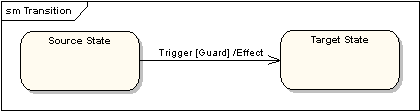
\includegraphics[width=7.5cm]{Bilder/sm6.png}
\caption{Transitions\cite{state_machine_diagram}}
\label{fig:transitions}
\end{minipage}
\begin{minipage}[t]{0.2\textwidth}
\centering
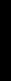
\includegraphics[width=0.3cm]{Bilder/join.png}
\caption{Fork and join}
\label{fig:fork}
\end{minipage}
\end{figure}

\textbf{Compound States}
There also exist sub-machine diagrams as shown in Figure
\ref{fig:compoundStates}.
\begin{figure}[ht]
    \centering
    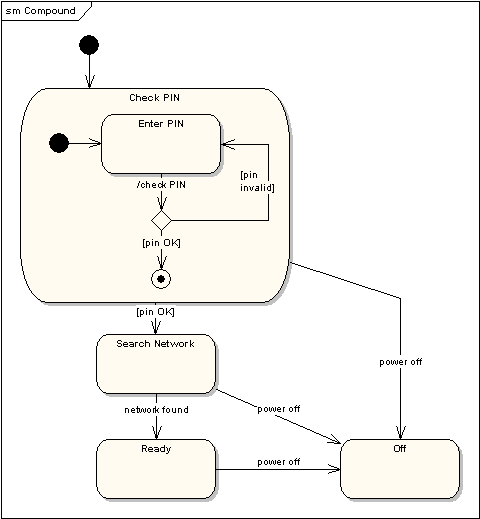
\includegraphics[scale=0.4]{Bilder/sm7.png}
    \caption{Compound States\cite{state_machine_diagram}}
    \label{fig:compoundStates}
\end{figure}

\textbf{Fork and Join}
As shown in Figure \ref{fig:fork} and \ref{fig:region}, fork and join are shown as a short thick bar that either branch into concurrent states or rejoin. 
The fork has one ingoing edge and multiple outgoing edges, while the join has multiple ingoing edges and one outgoing edge.

\textbf{Concurrent Regions}
The state can be divided into regions. The exit and execution can occur currently.
\begin{figure}[ht]
    \centering
    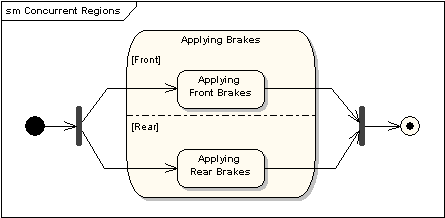
\includegraphics[scale=0.55]{Bilder/sm8.png}
    \caption{Concurrent Regions\cite{state_machine_diagram}}
    \label{fig:region}
\end{figure}

\section{ UML State Diagram constructor in Haskell}
\label{sec:UML state Diagram}
In this section, we explain the data type representation of the UML state diagram in Haskell in previous work by Junhao Tan \cite{jun_hao_tan}.
The type constructor \verb|UMLStateDiagram| has six types of data constructors.
And the outermost layer of a state diagram must be a sequential composite diagram.
The \verb|StateDiagram| constructor represents sequential composite states, 
the \verb|CombineDiagram| constructor represents concurrent composite states, 
the \verb|Joint| constructor represents join and fork,
the \verb|History| constructor represents the history node, 
the \verb|InnerMostState| constructor represents the states which contains no substates. 
The \verb|EndState| constructor represents the final states, and the initial states will be defined in \verb|StateDiagram| constructor as \verb|startState|.
   
\begin{verbatim}
type UMLStateDiagram = StateDiagram [Connection]

data StateDiagram a = 
  StateDiagram { substate :: [StateDiagram a],
                    label :: Int,
                    name  :: String,
                    connection :: a,
                    startState :: [Int]
                  }
 | CombineDiagram { substate :: [StateDiagram a],
                    label :: Int
                  }
 | EndState {
     label :: Int
     }
 | Joint { label :: Int
         }
 | History { label :: Int,
             historyType :: HistoryType
           }
 | InnerMostState { label :: Int,
                    name :: String,
                    operations :: String
                  }
deriving (Eq, Functor, Foldable, Show, Traversable)
\end{verbatim}

Each constructor in \verb|UMLStateDiagram| has a label that defines an element uniquely at the same level.
\verb|StateDiagram| has a substate list, a name, a connection list and an integer list that defines the initial state of a state diagram. The connection list lists transitions with a source state, a target state and an action.
For \verb|CombineDiagram|,it has a substate list in which there could only be \verb|StateDiagrams| and at least two \verb|StateDiagrams|.
For \verb|EndState| and \verb|Joint| ,there is no other parameter except the label.
\verb|History| has one parameter called \verb|historyType| which is either \verb|Deep| or \verb|Shallow|.
For \verb|InnerMostState|, it has a name of the state and an optional operations parameter that represents internal behaviours.

Here are some valid instances of state diagram expressions and the corresponding diagrams outputted through our drawing tool.

\begin{verbatim}
picture1 :: UMLStateDiagram
picture1 = StateDiagram [a,b] 1 "" [Connection[1] [2] "t",
           Connection[2] [1,3] ""] []
  where
    a = StateDiagram  [c,d,e] 1 "Composite State" [
        Connection [1] [2] ""] [1]
        where
         c = InnerMostState  1 "State 1" ""
         d = StateDiagram  [f,g] 2 "state 2" [
             Connection [1] [2] ""] [1]
          where
            f = InnerMostState  1 "State 2a" ""
            g = InnerMostState  2 "State 2b" ""
         e = History 3 Deep
    b = InnerMostState  2 "State 3" ""
\end{verbatim}

\begin{figure}[ht]
    \centering
    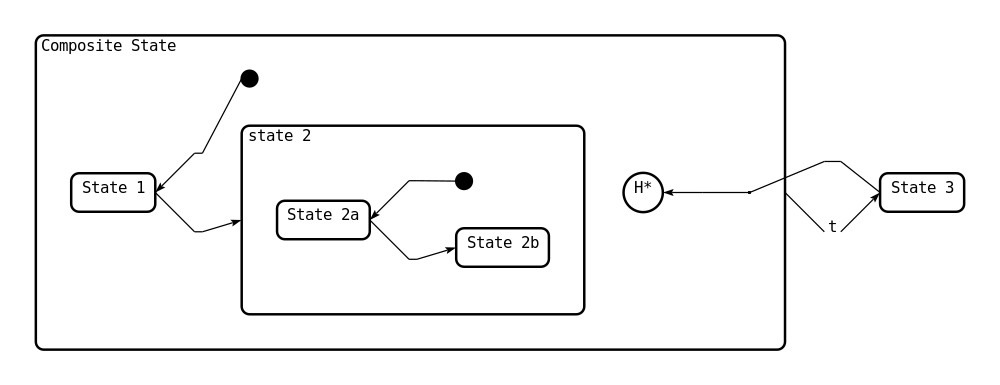
\includegraphics[scale=0.40]{Bilder/picture4.png}
    \caption{picture1}
    \label{fig:picture1}
\end{figure}

\newpage
\begin{verbatim}
picture2 :: UMLStateDiagram
picture2 = StateDiagram [a, b, c, d, l] 1 "" [Connection [1] [2] "a",
           Connection [2, 1, 2] [4] "h", Connection [2, 1, 3] [3] "",
           Connection [2, 2, 2] [3] "", Connection [3] [4] "g",
           Connection [4] [5] ""] [1]
  where
    a = InnerMostState 1 "A" ""
    b = CombineDiagram [e, f] 2
      where
        e = StateDiagram [g, h, i] 1 "" [Connection [1] [2] "b", 
            Connection [2] [3] "c"] [1]
          where
            g = InnerMostState 1 "B" ""
            h = InnerMostState 2 "C" ""
            i = InnerMostState 3 "D" ""
        f = StateDiagram [j, k] 2 "" [Connection [1] [2] "e"] [1]
          where
            j = InnerMostState 1 "E" ""
            k = InnerMostState 2 "F" ""
    c = Joint 3
    d = InnerMostState 4 "G" ""
    l = EndState 5
\end{verbatim}
        
\begin{figure}[ht]
    \centering
    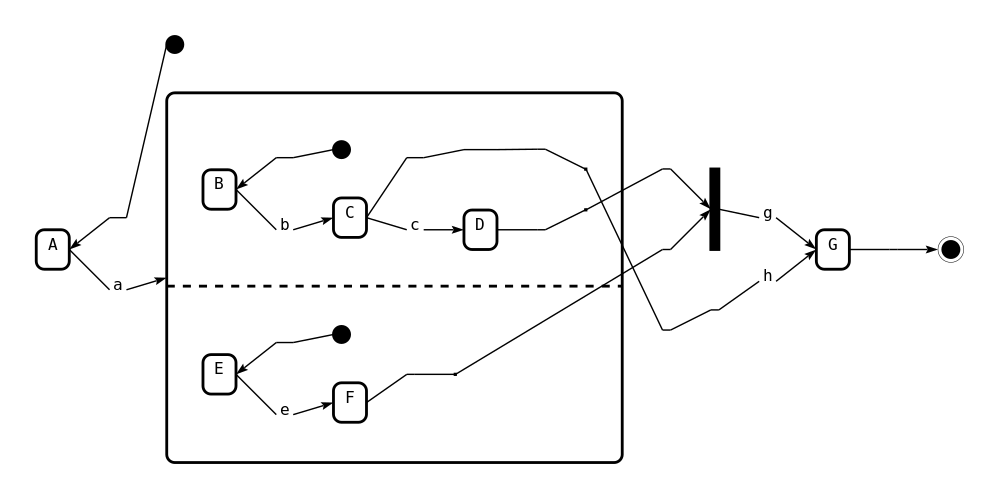
\includegraphics[scale=0.40]{Bilder/slide279.png}
    \caption{picture2}
    \label{fig:picture2}
\end{figure}
In the process of defining properties for a valid expression, we wonder users may input unexpected connections, so we defined two new functions, \verb|localise| and \verb|globalise| in the file of \verb|Datatype|.
Localizing is to transfer connections that are defined globally to local connections. Globalising is to pull all the connections to the outermost layer.
here \verb|[Connection[1,1] [1,2] ""]| is a more global description compared to \verb|[Connection [1] [2] ""]|.
\begin{verbatim}
sample :: UMLStateDiagram
sample = StateDiagram [a,b] 1 "" [Connection[1,1] [1,2] ""] [2]
     wheren
      a = StateDiagram  [c,d] 1 "" [Connection [1] [2] ""] [1]
          where
           c = InnerMostState 1 "A" ""
           d = InnerMostState 2 "B" ""
      b = InnerMostState  2 "C" ""
\end{verbatim}
\newpage

\section{Explanation of existing checkers}
\label{sec:existingCheckers}
Except for the previous presented \verb|UMLStateDiagram| inputs, we still need checkers to ensure that the hand inputs or randomly generated expressions of \verb|UMLStateDiagram| are valid or make sense. 
Hence, we need a thoroughly model-checking tool.
In Jun Hao Tan's thesis \cite{jun_hao_tan}, there already exist two basic checkers called \verb|checkValidity| and \verb|checkWrapper|.

The \verb|checkStructure| limits that none of the diagrams should violate these three properties.
\begin{itemize}
\item  The state machine diagram's outermost layer must be the \verb|StateDiagram|.
\end{itemize}
\begin{itemize}
\item  The \verb|CombineDiagram| constructor must contain at least two \verb|StateDiagram| and no other constructors.
\end{itemize}
\begin{itemize}
\item  The substates of \verb|StateDiagram| constructor cannot be empty or just \verb|History|/ \verb|Joint|.
\end{itemize}

 
The \verb|checkWrapper| defines four properties that must be fulfilled when drawing the diagram:
\begin{itemize}
\item The outermost layer must be the \verb|OrDecom| constructor
\end{itemize}
\begin{itemize}
\item  Substate of \verb|OrDecom| constructor cannot be empty or just \verb|Hist|/ \verb|For|/ \verb|StartS|/ \verb|Dummy|/ \verb|Transition|
\end{itemize}
\begin{itemize}
\item \verb|AndDecom| constructor must contain at least 2 \verb|OrDecom| and no other type of constructor.
\end{itemize}
\begin{itemize}
\item Horizontal slicing must be followed by vertical layering or vise visa
\end{itemize}

Here are counterexamples that the \verb|checkStructure| will reject.

The example \verb|forCheckOuterMostLayer| violates that the outermost layer must be the \verb|StateDiagram|.
Its outer layer is a \verb|CombineDiagram| instead, which is not allowed and will cause a blank \verb|.svg| file while outputting it.

\begin{verbatim}
forCheckOuterMostLayer :: UMLStateDiagram
forCheckOuterMostLayer = CombineDiagram [a,b] 1
     where
        a = StateDiagram  [InnerMostState 1 "A" ""] 1 ""  [] [1]
        b = StateDiagram  [InnerMostState 1 "B" ""] 2 ""  [] [1]
\end{verbatim}

In the \verb|forCheckSubstateSD|, the substrate of \verb|StateDiagram| contains only \verb|History|, violates that the substate of \verb|StateDiagram| constructor cannot be empty or just \verb|History|/ \verb|Joint|.

\begin{verbatim}
forCheckSubstateSD::UMLStateDiagram
forCheckSubstateSD = StateDiagram [a] 1 "" [] [1]
    where
        a = History 1 Deep
\end{verbatim}

Here \verb|forCheckSubstateCD| has only one element \verb|StateDiagram| as substate, violates that the \verb|CombineDiagram| constructor contains at least two \verb|StateDiagrams| and no other constructors.

\begin{verbatim}
forCheckSubstateCD :: UMLStateDiagram
forCheckSubstateCD = StateDiagram [CombineDiagram [a] 1] 1 "" [] []
    where
    a = StateDiagram  [InnerMostState 1 "A" ""] 1 ""  [] [1]
\end{verbatim}


In the further exploring, we split \verb|checkValidity| to two functions \verb|checkRepresatation| and \verb|checkStructure| and add further more testings like verify if outgoing edges from a history node always have the empty transition,the connection points or start points are valid,etc.
We will explain more specifically in a later section \ref{sec:properties}.



\section{ QuickCheck}
\verb|QuickCheck| \cite{claessen_hughes_2000} is a tool used to help programmers formulate and test the properties of programs. 
Properties are defined in Haskell functions and automatically checked on arbitrary inputs.
And a custom-made data generator is also possible to be defined.

If all the randomly generated or hand-input test cases pass the testing, 
it will report "\verb|OK|".
\begin{verbatim}
    +++ OK, passed 100 tests.
\end{verbatim}
Here are some functions we will use in the random inputs generator. 
More detailed examples and information could see \cite{quickcheck}.
\verb|data Gen a| is a generator for values of type \verb|a| \cite{quickcheck}.

If we define a data type of binary tree and do not want to choose a \verb|Leaf| too often,
we can use \verb|frequency| with a reasonale weighted distribution.
Our state diagram datatype could be seen as a tree.
Those states that contain no substates could be \verb|Leaf|.
\begin{verbatim}
    data Tree a = Leaf | Node (Tree a) a (Tree a)
    
    frequency :: [(Int, Gen a)] -> Gen   
\end{verbatim}
\verb|choose| is used to select a random one in the range of two elements.
\begin{verbatim}
    choose :: Random a => (a, a) -> Gen a  
\end{verbatim}
\verb|elements| is similar to \verb|choose|,
but the range of selection could be at arbitrary length but must be non-empty.
\begin{verbatim}
    elements :: [a] -> Gen a 
\end{verbatim}
This function \verb|vectorOf| is used to produce a list of the given length.
\begin{verbatim}
    vectorOf :: Int -> Gen a -> Gen [a]  
\end{verbatim}



\chapter{Implementation}
\label{chap:implementation}

\section{Structural checking}
\label{sec:properties}

Except for the existing checkers, we still have many invariants that were not checked.

\subsection{Diagram Representation}
\label{sec:representation}


First of all, the diagram expressions are either inputted by users or automatic generated must be valid.
There are several rules to define whether it is a representable diagram for our UML State diagram drawing tool.
The first two rules are already mentioned in section\ref{sec:existingCheckers}, which we will not further explain.


\begin{itemize}
\item  The outermost layer must be a state diagram instead of concurrent composite states.
\end{itemize}


\begin{itemize}
\item Concurrent composite states must contain at least two state diagrams and no other type of pseudostates.
\end{itemize}

\begin{itemize}
\item The beginning or endpoint of a transition should be a legal point. 
\end{itemize}

\begin{itemize}
\item The beginning or endpoint of a transition should not be empty.
\end{itemize}
\begin{itemize}
\item A transition should not go into or from a region of a concurrent composite state.

\end{itemize}
\begin{itemize}
\item The initial pseudostate of a state diagram should be a legal point.
\end{itemize}

\begin{itemize}
\item The initial pseudostate of a state diagram should not go into a region of a concurrent composite state.
\end{itemize}

We demonstrate some \verb|UMLStateDiagram| expressions that violate these properties.

The starting point of transition \verb|Connection [5] [1] "a"| in the \verb|forCheckConnection| does not exist in the substates. 
There are only two substates with labels 1 and  2, with no substates with label 5.
It violates the rule that the connection points must be valid.
\begin{verbatim}
forCheckConnection :: UMLStateDiagram
forCheckConnection = StateDiagram [a, b] 1 "" [
                     Connection [5] [1] "a"] [2]
  where
    a = InnerMostState 1 "A" ""
    b = InnerMostState 2 "B" ""
\end{verbatim}

In the \verb|forCheckEmptyConnPoint|, \verb|Connection[] [1] "a"| should not have a empty source state.
\begin{verbatim}
forCheckEmptyConnPoint :: UMLStateDiagram
forCheckEmptyConnPoint = StateDiagram [a,b] 1 "" [
                         Connection[] [1] "a"] [2]
     where a = InnerMostState  1 "A" ""
           b = InnerMostState  2 "B" ""
\end{verbatim}

The list \verb|[1,3]| in \verb|Connection [1,3] [2] ""| represents a state diagram with label 3 inside a concurrent composite state with label 1 which is a region.
It is not allowed to have connections with regions .
\begin{verbatim}
forCheckConnFromToRegion ::UMLStateDiagram
forCheckConnFromToRegion = StateDiagram [CombineDiagram [a,b] 1,
  InnerMostState  2 "" ""] 0 "" [Connection [1,3] [2] ""] []
    where
      a = StateDiagram [InnerMostState 0 "" ""] 3 "" [] [0]
      b = StateDiagram [InnerMostState 0 "" ""] 4 "" [] [0] 
\end{verbatim}

In the expression \verb|forCheckSubS|,the ininitial state \verb|[1,2]|  defined in a \verb|StateDiagram| does not exist.
There is only one state with label 1.
\begin{verbatim}
forCheckSubS :: UMLStateDiagram
forCheckSubS = StateDiagram [InnerMostState 1 "" ""] 1 "" [] [1,2] 
\end{verbatim}

The initial state \verb|[1,3]| in the example \verb|forCheckStartToRegion| denotes the \verb|StateDiagram| with label 3 inside a \verb|CombineDiagram| with label 1.
It is also a region that is not permitted by the defining properties.
\begin{verbatim}
forCheckStartToRegion ::UMLStateDiagram
forCheckStartToRegion = StateDiagram [CombineDiagram [a,b] 1,
 InnerMostState  2 "" ""] 0 "" [Connection [1,3,0] [2] ""] [1,3]
    where
      a = StateDiagram [InnerMostState 0 "" ""] 3 "" [] [0]
      b = StateDiagram [InnerMostState 0 "" ""] 4 "" [] [0] 
\end{verbatim}




\subsection{Diagram Structure}
\label{sec:structure}
Another aspect that needs to ensure is structure. The first constraint is already mentioned in section\ref{sec:existingCheckers}, which we will not further explain.
\begin{itemize}
\item The substates of a state diagram cannot be empty or only contains history, fork and join.
\end{itemize}
\begin{itemize}
\item Outgoing edges from a history node always have an empty transition description.
\end{itemize}
\begin{itemize}
\item Part of reachability: Excluding concurrent composite states and state diagram, all the nodes that are states, final states, history, fork and join, should be designated as a start state or be reached by a connection.
\end{itemize}

We show some counterexamples. 
In the example \verb|forCheckHistOutTransition|, the connection between \verb|History 1 Deep| and \verb|InnerMostState  2 "A" ""|  has an non-empty transition string.
It violates rule 2.
In the expression \verb|forCheckReachablity|, \verb| InnerMostState 1 "A" ""| is neither a initial state nor reached by other states.So this state is unreachable under our definition of reachability.
\begin{verbatim}
forCheckHistOutTransition :: UMLStateDiagram
forCheckHistOutTransition = StateDiagram [a,b] 1 "" [Connection[1] [2] 
                            "error"] [1]
     where
      a = History 1 Deep
      b = InnerMostState  2 "A" ""

forCheckReachablity :: UMLStateDiagram
forCheckReachablity = StateDiagram [a] 1 "" [] []
  where
    a = InnerMostState 1 "A" ""
\end{verbatim}




\subsection{Label Uniqueness}
\label{sec:representation}
Since we will assign a number to each component in the diagram, the uniqueness of these identifications of direct substates of a state diagram or composite states is essential.

It is not allowed to use the same labels at the same layer. In the diagram expression \verb|forCheckUniqueness|, \verb|InnerMostState|s have the identical label 1.
\begin{verbatim}
forCheckUniqueness :: UMLStateDiagram
forCheckUniqueness = StateDiagram [a, b] 1 "" [] [1]
  where
    a = InnerMostState 1 "A" ""
    b = InnerMostState 1 "B" "" 
\end{verbatim}



\subsection{Name Uniqueness}
\label{sec:representation}
Similarly, the criterion of label uniqueness could also be applied to local name uniqueness.
But additionally, to have a meaningful interpretation of the diagrams from a "user perspective", no state diagram should have the same name as one of its (possibly transitive) substates. 
An empty name of a state diagram will not be considered here.

For example,in the picture \ref{fig:nameUniq}, the three \verb|C|s conflict because the others are "inside"  the state diagram C.

\begin{figure}[ht]
    \centering
    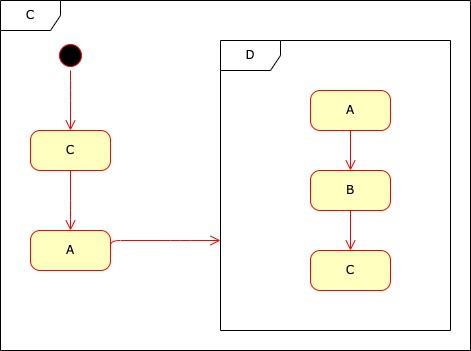
\includegraphics[scale=0.50]{Bilder/nameUniq.jpg}
    \caption{Name Uniqueness}
    \label{fig:nameUniq}
\end{figure}

In \verb|forCheckSDNameUniq|,  two state diagrams, one is inside the other, are named with identical string \verb|A|. It will misleading users. 
Similar in \verb|forCheckSubNameUniq|,  two \verb|InnerMostState|s conflict with each other,  with the same name.

\begin{verbatim}
forCheckSDNameUniq :: UMLStateDiagram
forCheckSDNameUniq = StateDiagram [a] 1 "A" [] []
     where
      a = StateDiagram  [InnerMostState  1 "B" ""] 1 "A" [] [1]

forCheckSubNameUniq :: UMLStateDiagram
forCheckSubNameUniq = StateDiagram [a,b] 1 "" [Connection[1] [2] ""] [1]
     where
      a = InnerMostState 1 "A" ""
      b = InnerMostState  2 "A" ""  
\end{verbatim}



\subsection{History States}
\label{sec:representation}
History nodes should never be reached by states inside their compound state and should only have connections towards their compound state.

We illustrate further by the following example \ref{fig:history}. 
The transitions from node \verb|A| and node \verb|E| to history are both valid. These two nodes are all inside history's compound state. However, the transitions from history to node \verb|B| and node \verb|F| are illegal because they are towards their compound state.

\begin{figure}[ht]
    \centering
    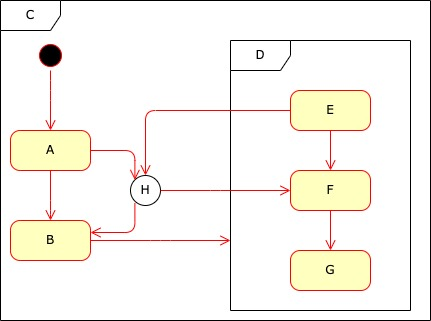
\includegraphics[scale=0.5]{Bilder/history.jpg}
    \caption{History}
    \label{fig:history}
\end{figure}

Here are some counterexamples. In \verb|forCheckInEdge|,  \verb|History 1 Deep| is reached by a connection that comes from its compound state. It is illegal.
In the expression \verb|forCheckOutEdge|, \verb|History 3 Deep| is incorrectly pointing to a state outside its compound state.
\begin{verbatim}
forCheckInEdge :: UMLStateDiagram
forCheckInEdge = StateDiagram [a,b] 1 "" [Connection [2] [1] ""] [2]
     where
      a =  History 1 Deep
      b = InnerMostState  2 "A" ""

forCheckOutEdge :: UMLStateDiagram
forCheckOutEdge2= StateDiagram [a,b] 1 "" [Connection [1,3] [2] ""
                  ] [1,3]
     where
     a = StateDiagram  [c,d] 1 "" [] [1]
          where
           c = InnerMostState  1 "A" ""
           d = History 3 Deep
     b = InnerMostState  2 "A" ""
\end{verbatim}



\subsection{Final States}
\label{sec:representation}
Final states should never have outgoing edges.
\begin{verbatim}
forCheckEndState :: UMLStateDiagram
forCheckEndState = StateDiagram [a,b] 1 "" [Connection[2] [1] ""] [2]
     where 
           a = InnerMostState  1 "A" ""
           b = EndState 2
\end{verbatim}
In the counterexample \verb|forCheckEndState|, the final state \verb|EndState 2| has a outgoing edge.



\subsection{Fork and Join}
\label{sec:representation}
For fork and join states, three aspects need to discuss.

\begin{enumerate}
\item \textbf{the number of ingoing and outgoing edges }

We divide this into two situations.
If a \verb|Joint| state is designated as a start state, that \verb|Joint| must have more than one outgoing edge and no other ingoing edges. 
If not, each Joint either has one ingoing edge and over one outgoing edge or has more than one outgoing edge and one ingoing edge.

\item  \textbf{the name of transitions}

 Analogous to the number of edges, we also have two cases. 
 If a \verb|Joint| state is also a start state, all transition strings of its outgoing connections should be empty.
 If not, it is not permitted that a \verb|Joint| state is reached by a connection with a non-empty transition string and is also left by a connection with a non-empty transition string.
 Moreover, all the ingoing edges to the same Joint should have the exact transition string, and all the outgoing edges from the same Joint should have the same transition string.
\item \textbf{connections to regions }

If several connections leave the same \verb|Joint| node, one of them must go to a distinct region.
If several connections reach the same \verb|Joint| node, one of them must come from a distinct region.
\end{enumerate}

We illustrate further with counterexamples.
\begin{verbatim}
forCheckMtoOne :: UMLStateDiagram
forCheckMtoOne = StateDiagram [a,b] 1 "" [Connection[5] [1,1,1] ""] [5]
      where
        a = CombineDiagram [e,f] 1
          where 
            e = StateDiagram [InnerMostState 1 "A" ""] 1 "" [] []
            f = StateDiagram [InnerMostState 1 "A" ""] 2 "" [] [1]
        b = Joint 5
\end{verbatim}
In this counterexample \verb|forCheckMtoOne|,the \verb|Joint 5| is also a start state,and should have more than one outgoing edges. However, in this expression, it has only one outgoing edge \verb|Connection[5] [1,1,1] ""|.

\begin{verbatim}
forCheckTransition :: UMLStateDiagram
forCheckTransition = StateDiagram [a,b] 1 "" 
 [Connection[5] [1,1,1] "a",Connection[5] [1,2,1] "b"] [5]
      where
        a = CombineDiagram [e,f] 1
          where 
            e = StateDiagram [InnerMostState 1 "A" ""] 1 "" [] []
            f = StateDiagram [InnerMostState 1 "A" ""] 2 "" [] []
        b = Joint 5
\end{verbatim}
In this counterexample \verb|forCheckTransition|,the \verb|Connection[5] [1,1,1] "a"| and \verb|Connection[5] [1,1,1] "a"| is connected with \verb|Joint 5| which is also a start state.
It is not allowed here to have non-empty and not identical transiton strings of these two connections.

\begin{verbatim}
forAllgoIntoParallelRegions :: UMLStateDiagram
forAllgoIntoParallelRegions = StateDiagram [a,b] 1 "" 
 [Connection[5] [1,1,1] "a",Connection[5] [1,1,2] "a"] [5]
      where
        a = CombineDiagram [e,f] 1
          where 
            e = StateDiagram [InnerMostState 1 "A" "",
              InnerMostState 2 "B" ""] 1 "" [] []
            f = StateDiagram [InnerMostState 1 "A" ""] 2 "" [] [1]
        b = Joint 5
\end{verbatim}

In this counterexample \verb|forAllgoIntoParallelRegions|,the \verb|Joint 5| has two outgoing edges connected two states from the same region. 

\begin{verbatim}
forAllcomeOutOfParallelRegions :: UMLStateDiagram
forAllcomeOutOfParallelRegions = StateDiagram [a,b] 1 "" 
 [Connection[1,1,1] [5] "a",Connection[1,1,2] [5] "a",
    Connection[5] [1,2,1] "a" ] [1,1,2]
      where
        a = CombineDiagram [e,f] 1
          where 
            e = StateDiagram [InnerMostState 1 "A" "",
              InnerMostState 2 "B" ""] 1 "" [] [1]
            f = StateDiagram [InnerMostState 1 "A" ""] 2 "" [] []
        b = Joint 5
\end{verbatim}

In this counterexample \verb|forAllcomeOutOfParallelRegions|,the \verb|Joint 5| is reached by two connections come from a identical region.




\subsection{Crossings between regions}
\label{sec:representation}
It is not allowed to have a transition that the starting point and the endpoint come from two different regions.

In a counterexample \verb|forCheckCrossings|, two states from two different regions of \verb|CombineDiagram [a,b] 1| are connected.
\begin{verbatim}
forCheckCrossings :: UMLStateDiagram 
forCheckCrossings = StateDiagram [CombineDiagram [a,b] 1] 0 ""
  [Connection [1,2,0] [1,3,0] ""] [1,2,0]
    where
      a = StateDiagram [InnerMostState 0 "" ""] 2 "" [] []
      b = StateDiagram [InnerMostState 0 "" ""] 3 "" [] []
\end{verbatim}


\subsection{Semantics}
\label{sec:semantics}
Except for errors by calling the drawing function, some UML diagrams do not make much sense. 
Here we have two limits on semantics checking and will explain them with corresponding counterexamples.
\begin{itemize}
\item No two connections can leave the same source and have the same label (except from a \verb|Joint| Node).
\end{itemize}
\begin{itemize}
\item The non-\verb|Joint| state, which has more than one outgoing connection, must have a non-empty transition label.
\end{itemize}

\begin{verbatim}
forCheckSameConnection :: UMLStateDiagram
forCheckSameConnection = StateDiagram [a, b] 1 "" 
 [Connection [1] [2] "a", Connection [1] [2] "a"] [1]
  where
    a = InnerMostState 1 "A" ""
    b = InnerMostState 2 "B" ""
\end{verbatim}
In the counterexample \verb|forCheckSameConnection|, \verb|Connection [1] [2] "a"| and \verb|Connection [1] [2] "a"| have the identical source state which is also not a \verb|Joint| node and have the same transition string.
It is not allowed to have the same string at this condition.

\begin{verbatim}
forCheckEmptyTran :: UMLStateDiagram
forCheckEmptyTran = StateDiagram [a, b] 1 "" 
 [Connection [1] [2] "a", Connection [1] [2] ""] [1]
  where
    a = InnerMostState 1 "A" ""
    b = InnerMostState 2 "B" ""
\end{verbatim}

Here \verb|Connection [1] [2] "a"| and \verb|Connection [1] [2] ""| have the identical source state which is also not a \verb|Joint| node but \verb|Connection [1] [2] ""| wrongly have an empty string here.






\section{Structural checking in Haskell}
\label{sec:concept}
This section illustrates how the testing properties defined in the previous are implemented as Haskell functions.

\textbf{Diagram Representation}

To verify the outermost layer is a state diagram, the function needs to check if the state at the first layer is a \verb|StateDiagram|. For the following two constraints, we have two parts to transversely check. All the substates of a combine diagram must have over one state diagram and no other constructors, and all the transitions have no empty starting or end point lists.

There are two general rules that the connections between elements must obey.
\begin{itemize}
\item The start node and the end node of one connection must be valid.
\item No connection could start from or end at regions themselves.
\end{itemize}

As defined in \verb|UMLStateDiagram|,only sequential composite states have connections.
At first, we get all the start points and endpoints of one sequential composite state.
Then we check each point list which could refer to one node in deeper level or this layer, by verifying if each element of the list is contained in further substates' label list.
To prevent connections starting or ending at regions, the last second node of the point list should not be \verb|CombineDiagram| since a region is a \verb|StateDiagram| inside the \verb|CombineDiagram|.
Then we check the connection points and start points layer by layer that does not violate the above condition.

The initial pseudostate constraints are similar to connections'. So the approaches are also similar.
\begin{itemize}
\item The point list must refer to a valid node in the diagram
\item No initial pseudostates could point to regions themselves
\end{itemize}
We verify that each element in one start point list is contained in the further substates' label list.
And only the composite state has substates, and only the sequential composite state has a \verb|startState| field.
To check the second rule, from the first element to the last second element of one start point list must be checked that it is not a concurrent composite state.

\textbf{Diagram Structure}

There are three functions to realize the testing of diagram structure.
In the function \verb|checkSubstateSD|, we transversely check the substates of all the \verb|StateDiagram| in the entire diagram if substates only have \verb|Joint| or \verb|History| states.
The function \verb|checkHistOutTransition| will verify transversely all the transitions in the connection list of each \verb|StateDiagram| that arrive at a \verb|History| node have empty strings.
The function \verb|checkReachablity| pulls all the connections to the outermost layer using \verb|globalise| function and collects all the elements that are not \verb|StateDiagram| or \verb|CombineDiagram|.
Then it also collects the source states of all the connections after globalizing, and all nodes that are the start states represented like at the outermost layer. We denote this list as C here.
Finally, suppose all the elements in the list of all the elements that are not \verb|StateDiagram| or \verb|CombineDiagram| are elements of the list C. In that case, we could say the expression satisfies reachability.

\textbf{Label Uniqueness}

The identifier of each state at the same layer must be unique.
We check the direct substates of each state diagram or combine diagrams if two substates have the same label.

\textbf{Name Uniqueness}

If the nodes all belong to the same \verb |StateDiagram|'s or \verb |CombineDiagram|'s substates, we say that these nodes are at the same layer.
At the same layer, states that have identical names are not acceptable.
And if deeper substates of one state diagram have identical names as the state diagram, it is also not valid.

We get all direct substates' names of a state diagram or a combined diagram and check for duplicates.
If there are duplicates, then the diagram violates the same layer uniqueness.

To prevent deeper layer name conflict, the name field of one state diagram needs to be compared to all arbitrarily deep substates' names includes its direct substate's name.
The name of them could not be equal.

\textbf{History States} 

The idea of checking if a history node is connected with states inside their compound states is to compare two point lists in a connection that starts or ends from/at a \verb |History| node.
We take the prefix of the other state of the same length as the \verb |History| state. 
Following this, the function compares if all the elements except the last one of these two lists are identical. 
If they are the same, we could say the history node points to a state inside its compound states in this transition.
For outgoing edges of a history node, the function needs to verify if all the elements except the last one of these two lists are non-identical.

\textbf{Final States}

As a final state, it should have no outgoing edges. It also means the start point of all connections should not be a final state. So we need to verify that the \verb|pointFrom| of each connection in each state diagram does not refer to an end state.

The function \verb|isNotEnd| takes an \verb|pointFrom| and \verb|UMLStateDiagram| as inputs.
Suppose the length of the integer list is longer than one. 
In that case, the function will find the substate inside the second argument \verb|UMLStateDiagram|'s direct substates with the same label as the first element of the input list 
and continue to take the tail of the list. 
The new substate as arguments to call \verb|isConnFromNotEnd| repeatedly until the length of the integer list is one.
When the length is one, we check if a label of substates of the diagram that is end-state has the same value as the only element in the list.
If that is not true, this point does not point to the end state.

\textbf{Fork and Join}

The key idea to realize this function is to globalize all the connections/ to the outermost layer using \verb|globlise| function or represent all the elements or start states like in the outermost layer.

To check the number of in/outgoing edges, we will filter all the connections of which the source state is \verb|Joint| state as a list of outgoing edges from \verb|History| 
and all the transitions of which the target state is \verb|Joint| state as a list of ingoing edges to \verb|History|.
Moreover, all the \verb|Joint| states that are designated as start states will be collected.
There are six illegal situations as illustrated in Figure \ref{fig:in/outgoing edges}.
After that, the list of all \verb|Joint| state that has over one outgoing edge will be compared to the list of all \verb|Joint| state that has over one ingoing edge.
This is not legal if there is an intersection between these two lists as shown in (1).
Secondly, It is not valid if the list of the \verb|Joint| states designated as start states intersects with the list of all \verb|Joint| states having ingoing edges.
As shown in (3), the list of the \verb|Joint| states designated as start states has intersections with the list of all \verb|Joint| states with only one outgoing edge.
This is also not permitted.
To avoid circumstance (4), the function will verify if all \verb|Joint| states with no ingoing edges are start states.
Similarly, the function will check if there are \verb|Joint| states have no outgoing edges to avoid the situation (5).
In the end, the list of all \verb|Joint| states with only one outgoing edge and the list of all \verb|Joint| states with only one ingoing edge will be evaluated whether there are intersections to avoid the situation (6).
\begin{figure}[ht]
    \centering
    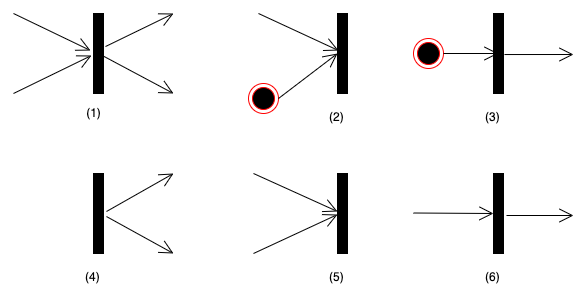
\includegraphics[scale=0.5]{Bilder/MtoOne.png}
    \caption{Illegal in/outgoing edges}
    \label{fig:in/outgoing edges}
\end{figure}

In Figure \ref{fig:Transition with illegal strings} there are four invalid situations.
Two extra functions with two parameters, connection and connection list, are defined to check if all the transitions strings are the same by filtering the connections with the same source state or target state as the first parameter.  
The function will check if all the elements in the list of connections with a \verb|Joint| as the source state or target state could pass those two extra functions to avoid situations (1), (2).
We also have to ensure that the list of \verb|Joint| states that have outgoing connections with non-empty strings have no intersections with the list of  \verb|Joint| states that have ingoing connections with non-empty strings as shown in (3).
Lastly, the start states that are \verb|Joint| states should not show in the list of  \verb|Joint| states that have outgoing connections with non-empty strings.
\begin{figure}[ht]
    \centering
    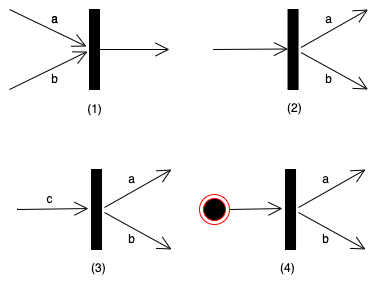
\includegraphics[scale=0.5]{Bilder/transitions.png}
    \caption{Transition with illegal strings}
    \label{fig:Transition with illegal strings}
\end{figure}

\textbf{Crossings between regions}

since the crossing problem was found in the process of creating the \verb|localise| and \verb|globalise| functions, those associations between regions will be eliminated after localising. 
We could compare the number of connections before and after localising. If the quantity is changed, there must have some illegal crossings between regions in the expression.

\textbf{Semantics} 

As an \verb|UMLStateDiagram|, it does not make much sense when those two criteria in section \ref{sec:semantics} are violated.

The strategy to check the first rule is to pull all the connections to the outermost layer of the diagram and filter those connections that do not have a \verb|Joint| node as the source state.
After that, we verify whether two associations have an identical source state and equal transition string.
An extra function \verb|checkSameOutTran| takes one connection and the entire connection list without \verb|Joint| states as inputs. 
Then it filters those connections that have the same start point and the same transition string as the first connection parameter. 
After that, if the length of the remaining connection list is equal to one, there are no violations when the source state is the same as the first parameter's.
Hence if all the connections in the list could pass the function \verb|checkSameOutTran|, the entire diagram expression must have satisfied the first rule.

The approach to the second rule is similar to the way shown above. 
The first step is to pull all the connections to the outermost layer of the diagram and filter those connections that do not have a \verb|Joint| node as the start point.
An extra function \verb|checkEmptyOutTran| takes one connection and the entire connection list without \verb|Joint| states as inputs. 
Then it filters those connections that have the same source state.
After that, if the length of the remaining connection list is equal to one or none of them has an empty transition string, there are no violations when the source state is the same as the first parameter's.
Hence if all the connections in the list could pass the function \verb|checkEmptyOutTran|, the entire diagram expression must have satisfied the second rule.






\section{Automatic test case generator }
\label{sec:generator}
This section presents an automatic test case generator for  UML state diagram using \verb|QuickCheck|.
This tester generates random graphs to monitor the UML Diagram drawing tool if there are exceptions.

In our current model, nested combine diagram which means a combine diagram inside another combine diagram will not occur.
Because it will cause the generator retry hundreds of times to satisfy the constraints which is not ideal for a quick testing and generation.
We might will improve this model to allow nested combine diagram in the future work.
Besides, self-edges is also ignored since the drawing tool has a issue with it.Moreover,semantics constraints are achieved by retries in our model,and only part of semantics constraints are specifically defined.

\subsection{randomSD}
Given is the implementation of \verb|randomSD|, We have some additional limitations on the diagram generating except for satisfying testing properties mentioned in the previous section.
\begin{itemize}
\item The depth of the diagram is controlled with a \verb|counter| argument which equals 4. In a branch, when a state diagram is produced, the counter will be reduced by one.
\end{itemize}
\begin{itemize}
\item We set \verb|cdMaxNum| to 1 to narrow the diagram sample down by excluding these with nested composite states. In other words, no composite states will be inside other composite states.
\end{itemize}
\begin{itemize}
\item The usage of the \verb|frequency| function specifies the probability of generating graphs with at least two levels.
\end{itemize}
\begin{verbatim}
randomSD :: Gen (UMLStateDiagram, Int)
randomSD = do
  let outermost = True
      counter = 4 
      ns = [3 .. 4]
      alphabet = ["A","B","C","D","E","F","G","H","I","J","K","L",
       "M","N","O","P","Q","R","S","T","U","V","W","X","Y"]
      l = 1
      mustCD = False
      cdMaxNum = 1 
  nm <- elements alphabet
  leastTwoLevels <- frequency [(2,return False),(8,return True)]
  randomSD' outermost counter cdMaxNum leastTwoLevels ns alphabet (l,
   nm,mustCD) [] 
\end{verbatim} 
The first argument of \verb|randomSD'|, \verb|True|, represents this state diagram is the outermost layer. 
In \verb|(1,nm,mustCD)|, \verb|nm| is chosen randomly as the name string of the state diagram,
the Integer 1 represents the label value, and \verb|mustCD| defines whether the substates of state diagram must contain a combine diagram. \verb|[3 .. 4]| is the number choice of substates. 
The element \verb|alphabet| is the name range for state diagram and \verb|InnerMostState|.
The empty list defines names that should not be used for substates at an arbitrary depth.



\subsection{randomSD'}
\label{subsec:randomSD'}
As we explained in section\ref{sec:UML state Diagram}, a \verb|StateDiagram| have five arguments: substate,label, name, connection, startState.

Let us decide substate list first. 
To generate substates, we will map each element of a tuple list to function \verb|randomInnerSD| (see section \ref{subsec:randomInnerSD} ), which has six parameters. 
The argument \verb|counter| will be reduced by one to control the depth of the entire diagram.
And the name list that should not be used inside will be added by one more string, the name of the current state diagram. It is used to prevent the naming confusion of states.
The choice of substates quantity, \verb|cdMaxNum| and name options for the whole graph will remain the same.
Here we illustrate how the tuple with four essential elements assigned to each substate is generated.
After arbitrarily choosing the number of substates as n, we will use the shuffle algorithm to generate a random permutated Integer list as labels with length n+1. 
The number of labels will exceed one because the function will add an extra \verb|combDiagram| substate if some conditions are not satisfied to achieve the necessity of containing a \verb|combDiagram| inside if \verb|mustCD| is True.
The second parameter of the tuple is the node types list (see the NodeType in \ref{subsec:randomInnerSD} ).
The combination of types of substates should mainly satisfy four rules :
\begin{itemize}
\item The number of history or final states should be less than 2.
\end{itemize}
\begin{itemize}
\item The number of \verb|CombDiagram| and \verb|StateDiagram| should be less than 3 to simplify our diagram model.
\end{itemize}
\begin{itemize}
\item If the generator arbitrarily decides the diagram must contain over two levels and \verb|outermost| is \verb|True|, \verb|CombDiagram| or\verb| StateDiagram| must be an element of substates.
\end{itemize}
\begin{itemize}
\item If all the substates have no states without substates, \verb|Joint| should not be an element of substates.
Besides, If \verb|cdMaxNum| equals zero, substates contain no \verb|Joint| and no \verb|CombDiagram|.
If \verb|counter| is greater than zero, all the substates should be states that have no substates.
\end{itemize}
If the substate type list contains \verb|Joint| and \verb|cdMaxNum| is not zero, we define a new element \verb|newMustCD| equals True.
If not, we assign the value \verb|mustCD| to \verb|newMustCD|.
We will use \verb|newMustCD| to ensure a combine diagram inside substates if \verb|newMustCD| is True.
There are three situations to discuss.
\begin{itemize}
\item If \verb|counter == 0| and  additionally \verb|newMustCD == True|, we must put an extra Comb element to the substate type list.
\end{itemize}
\begin{itemize}
\item If \verb|newMustCD == False|, we have no requirement to contain \verb|Comb| in the \verb|subTypes|, so \verb|subTypes| will remain the same. Moreover, each value in the \verb|mustCD| list will be set to \verb|False| for the recursive calls.
\end{itemize}
\begin{itemize}
\item If \verb|counter > 0| and \verb|newMustCD == True|,  we can randomly choose whether to create a leaf or branch. But there are some constraints:
\begin{enumerate}
\item If there is no combine diagrams or no state diagrams in substates, we must put an extra \verb|Comb| element to \verb|subTypes| because we won't have another chance to produce that combine diagram. Then we will set the whole \verb|mustCD| list to False since there is a combine diagram.
\item If there is combine diagrams in substates, no addition on \verb|subTypes| and the whole \verb|mustCD| list to False.
\item If there is no combine diagrams but a state diagram, we must ensure that combine diagrams will occur somewhere deeper in the tree. So we flip a coin to choose which state diagram in the substates must contains a combine diagram.
\end{enumerate}
\end{itemize}
After that, we use \verb|zip4| functio to make a list of tuples, each tuple containing elements of four lists occurring at the same position and map them to each \verb|randomInnerSD| call to generate substates list.

Secondly, the start state will be randomly chosen in the range of all the elements inside the current state diagram. But no two start states can point to the same node. All the nodes that have been chosen as start states in deeper levels will be discarded. We also limit the frequency of selecting direct substates and components inside substates with 
\begin{verbatim}
frequency 
    [(2, elements (innerElemNoRegions \\ globalStartsWithoutCurrent))
       ,(8,elements layerElem)]
\end{verbatim}
Lastly, transitions generation will be divided into two situations.
If this is not at the outermost layer, only components that are not  \verb|Joint| will have connections because we only can satisfy the constraints to  \verb|Joint| nodes at the outermost layer. 
The selection range of the source state is all the components without type of final states.
The target state should not be a history node that is a direct substate of the current state diagram and not be an element in a parallel region of the source state. 
Besides, there is an issue to draw self-edges in the current drawing tool, so we will not contain self-edges in our model.
Since a natural diagram, connections are most between the same layer, we adjust the probability of choosing direct substates and more inner elements like we did as start states. But if the inner elements list is empty, which means this is the end of this branch, only layer elements are possible.
We also limit the transition strings that should not be the same as other transitions starting from the same node, and if there is another connection starting from the same node, the string should not be empty.
Nevertheless, there are some exceptions that we need to regenerate the source state or the target state. The constraints that no connections start and end at two different regions must also be satisfied here.
\begin{itemize}
\item If the starting point is history node, the endpoint must be inside the compound states of the starting point, and the transition string should be empty.
\end{itemize}
\begin{itemize}
\item If the endpoint is history node, the starting point must be outside the compound states of the endpoint. If the newly generated starting point is also a history node, the transition string will be reassigned to empty.
\end{itemize}


If this is the outermost layer, we must make relations for all the \verb|Joint| nodes after transitions between \verb|non-Joint| components are arbitrarily produced.
As we mentioned in the section, a \verb|Joint| node should only have over one outgoing edge and one ingoing edge or above one ingoing edge and one outgoing edge. So firstly, we will randomly choose the number of outgoing edges, either one or two, then decide the number of ingoing edges. But if the \verb|joint| state is also a start state, the number must be two, and no other ingoing edges will be generated.
The options for states connected to a \verb|Joint| node is the elements under one combine diagram. In the entire diagram, there maybe have several combine diagrams, but we will randomly select one and take their inside components as selection range.
Moreover, if the number of connections at one side of a \verb|Joint| state is over one, there must be at least one state from a different region of the other.
Besides, the starting point of connection still should not be a final state, and we eliminate duplicate links with the same source state and target state here.
Concerning transition strings, we will set the transitions at one side of  \verb|Joint| with the identical string or both empty. If the string is not empty at one side, the other side string must be empty.

Furthermore, since all the connections are arbitrarily produced, we could not ensure that all states are reachable. Extra relations of those unreachable states should be created.

So finally, the connection list is the combination of these three parts. If this is not the outermost layer, the extra connections and \verb|Joint| connections will be empty.

\subsection{randomInnerSD}
\label{subsec:randomInnerSD}
We define a datatype \verb|NodeType| to represent the type of states in the UML state diagram.
Given is the implementation of \verb|randomInnerSD|, we call this function only in \verb|randomSD'| (see section \ref{subsec:randomSD'}) to generate substates.

It has six arguments. 
The variable \verb|counter| and \verb|cdMaxNum| could control the depth and the number of current composite states in a branch but not be changed in this function only pass them to function \verb|randomCD| or \verb|randomSD'|.
\verb|ns| and \verb|alphabet| are the number options of substates and name choices for the entire diagram.
The fifth arguments is a tuple,\verb|(l,t,s,mustCD)| with type\verb| (Int,NodeType,[String],Bool)|. \verb|l| is the label.
\verb|t|, which is a NodeType indicates the type of states.
String list s is the names assigned to the states. 
Only if the node is \verb|Comb| type which represents combine diagrams, the length of the string list will be over one(see section \ref{subsec:randomSD'}).
We use \verb|mustCD| to tell if a current composite state is a must in this branch.
\verb|exclude| is the name list that should not be utilized on deeper levels.

According to the value of \verb|t|, the function will return the corresponding type of states.
For the sequential composite states, the value of outermost will be automated set to False.

\begin{verbatim}
data NodeType = Hist | End | Inner | Comb | Stat | Join  deriving Eq
\end{verbatim}

\begin{verbatim}
randomInnerSD::Int -> Int -> [Int] -> [String] ->
(Int,NodeType,[String],Bool) -> [String] -> Gen UMLStateDiagram
randomInnerSD counter cdMaxNum ns alphabet (l,t,s,mustCD) exclude = do
 let nm = head s
 case t of 
  Hist -> 
   frequency 
    [(1,return (History l Shallow)),(1,return (History l Deep))]
  End -> return (EndState l)
  Inner -> return (InnerMostState l nm "")
  Comb -> randomCD counter cdMaxNum ns alphabet l s exclude
  Stat -> 
   randomSD' False counter cdMaxNum False ns alphabet (l,nm,
      mustCD) exclude
  Join -> return (Joint l)
\end{verbatim}




\subsection{randomCD}
\label{subsec:randomCD}
In this section, we present how to generate arbitrarily concurrent composite states. 
\verb|CombineDiagram| consists of two parameters, an Integer called label and substate.

Firstly, the function randomly decides the number of substates between 2 and 3 and assigns values to the \verb|StateDiagram| generator.
Because of the constraints in section \ref{sec:representation}, concurrent composite states should only contain sequential composite states, and the number must be over two.
\verb|cdMaxNum| is reduced by one because we simplify the model not containing nested combine diagrams.
And the necessity to have combine diagrams in deeper levels will be False. The \verb|exlude| parameter will not be changed since combine diagrams has no name.
And \verb|outermost| will be False since it is not the outermost layer. 
The arguments \verb|s| is a name list assigned for substates from the previous layer.

At last, the function returns a combine diagrams with label \verb|l| reserved from the previous \verb|randomSD| call and the produced substate list here.
\begin{verbatim}
randomCD :: Int -> Int -> [Int]-> [String] -> Int -> [String] ->
  [String] -> Gen UMLStateDiagram
randomCD counter cdMaxNum ns alphabet l s exclude = do
 n      <- elements [2 .. 3]
 labels <- shuffle [1..n]
 let cdMaxNum' = cdMaxNum - 1
     mustCDs =replicate n False
     cond   = zip3 labels s mustCDs
 subs <- mapM 
   (\x ->
     randomSD' False counter cdMaxNum' False ns alphabet x exclude) cond
 return (CombineDiagram subs l)
\end{verbatim}



\chapter{Evaluation}
\label{chap:evaluation}
\section{Fuzzing and Results}
Fuzz test is an automated software testing approach feeding inputs to target programs to expose vulnerabilities and fix them in advance. Compared to other vulnerability discovery techniques, the fuzzing test has high accuracy and good scalability.  
Our fuzzing test is based on known data structures and measuring the code coverage, so it is a generation-based and coverage-based fuzzer.\cite{li_zhao_zhang_2018}

Figure \ref{fig:fuzzing} shows the process of fuzzing tests which consists of four main parts, testcase generation, program implementation, program monitoring and violation analysis. So the quality of test cases significantly impacts the testing effects. The inputs should satisfy the properties of data structures as much as possible and, on the other hand, should be wide enough to reveal problems embedded in the software. \cite{li_zhao_zhang_2018}
\begin{figure}[ht]
    \centering
    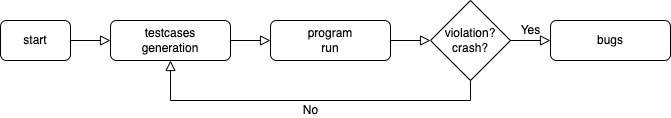
\includegraphics[scale=0.4]{Bilder/fuzz.png}
    \caption{process of fuzzing test}
    \label{fig:fuzzing}
\end{figure}

As the implementation depicted in the section \ref {sec:generator}, our random input generator could satisfy all the testing properties we proposed before and are forced to generate diagrams with \verb|Joint| and at least two levels with great possibility. 
It could generate many and different diagram expressions that even we might have never tried by hand and very rare. 

We take some random data as inputs to our exiting drawing tool. 
Here are some results. The generated component types and transitions in a diagram expression achieve high randomness.

 
\begin{figure}[htbp]
\centering
\begin{minipage}[t]{0.4\textwidth}
\centering
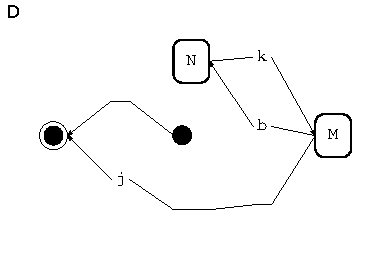
\includegraphics[width=5.5cm]{Bilder/sample3.pdf}
\caption{sample 1}
\end{minipage}
\begin{minipage}[t]{0.4\textwidth}
\centering
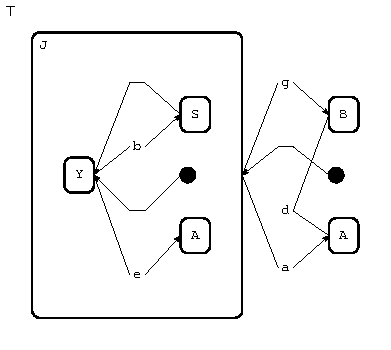
\includegraphics[width=5.5cm]{Bilder/sample1.pdf}
\caption{sample 2}
\end{minipage}
\end{figure}

\begin{figure}[htbp]
\centering
\begin{minipage}[t]{0.48\textwidth}
\centering
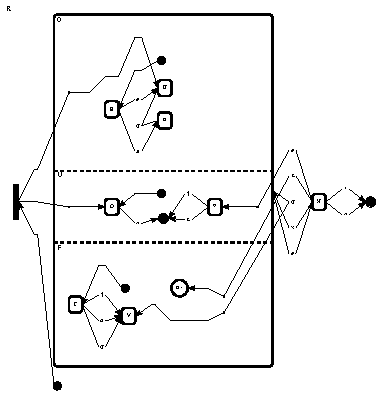
\includegraphics[width=6cm]{Bilder/sample4.pdf}
\caption{sample 3}
\end{minipage}
\begin{minipage}[t]{0.48\textwidth}
\centering
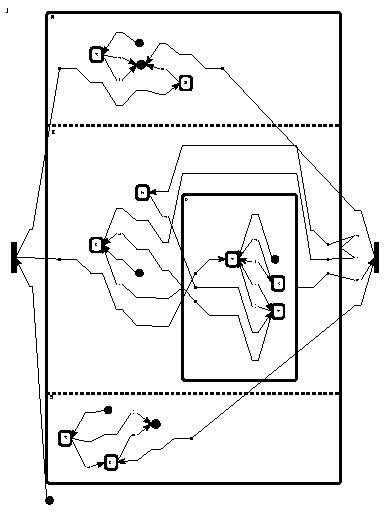
\includegraphics[width=6cm]{Bilder/sample2.pdf}
\caption{sample 4}
\end{minipage}
\end{figure}

After several experimental executions, we found our drawing tool crashed in certain situations and will show two types of errors :

\begin{verbatim}
 sampling.exe: Maybe.fromJust: Nothing
\end{verbatim}
\begin{verbatim}
 sampling: No match in record selector lengthXY
\end{verbatim}

Those errors may be fixed in later work. Here we simply ignore those diagrams that the tool are unable to draw.
The fuzzing test eventually helps us improve the program since our random generator will produce many corner cases that may cause the program to fail.


\section{Coverage Analysis}

 We use the HPC toolkit \cite{gill_runciman_2007} to measure the degree of thoroughness of our test suite.
Figure \ref{fig:coverage1} and \ref{fig:coverage2} gives the code coverage of each module. 

From the code coverage measured by HPC, the average coverage of the top-level definitions is 91$\%$. It is an ideal result since it is reasonable that some codes would not be executed\cite{gill_runciman_2007}.
We have achieved very high coverage on checkers.
However, the coverage on the arrow drawing is deficient.
This could be our future focus.

\begin{figure}[ht]
    \centering
    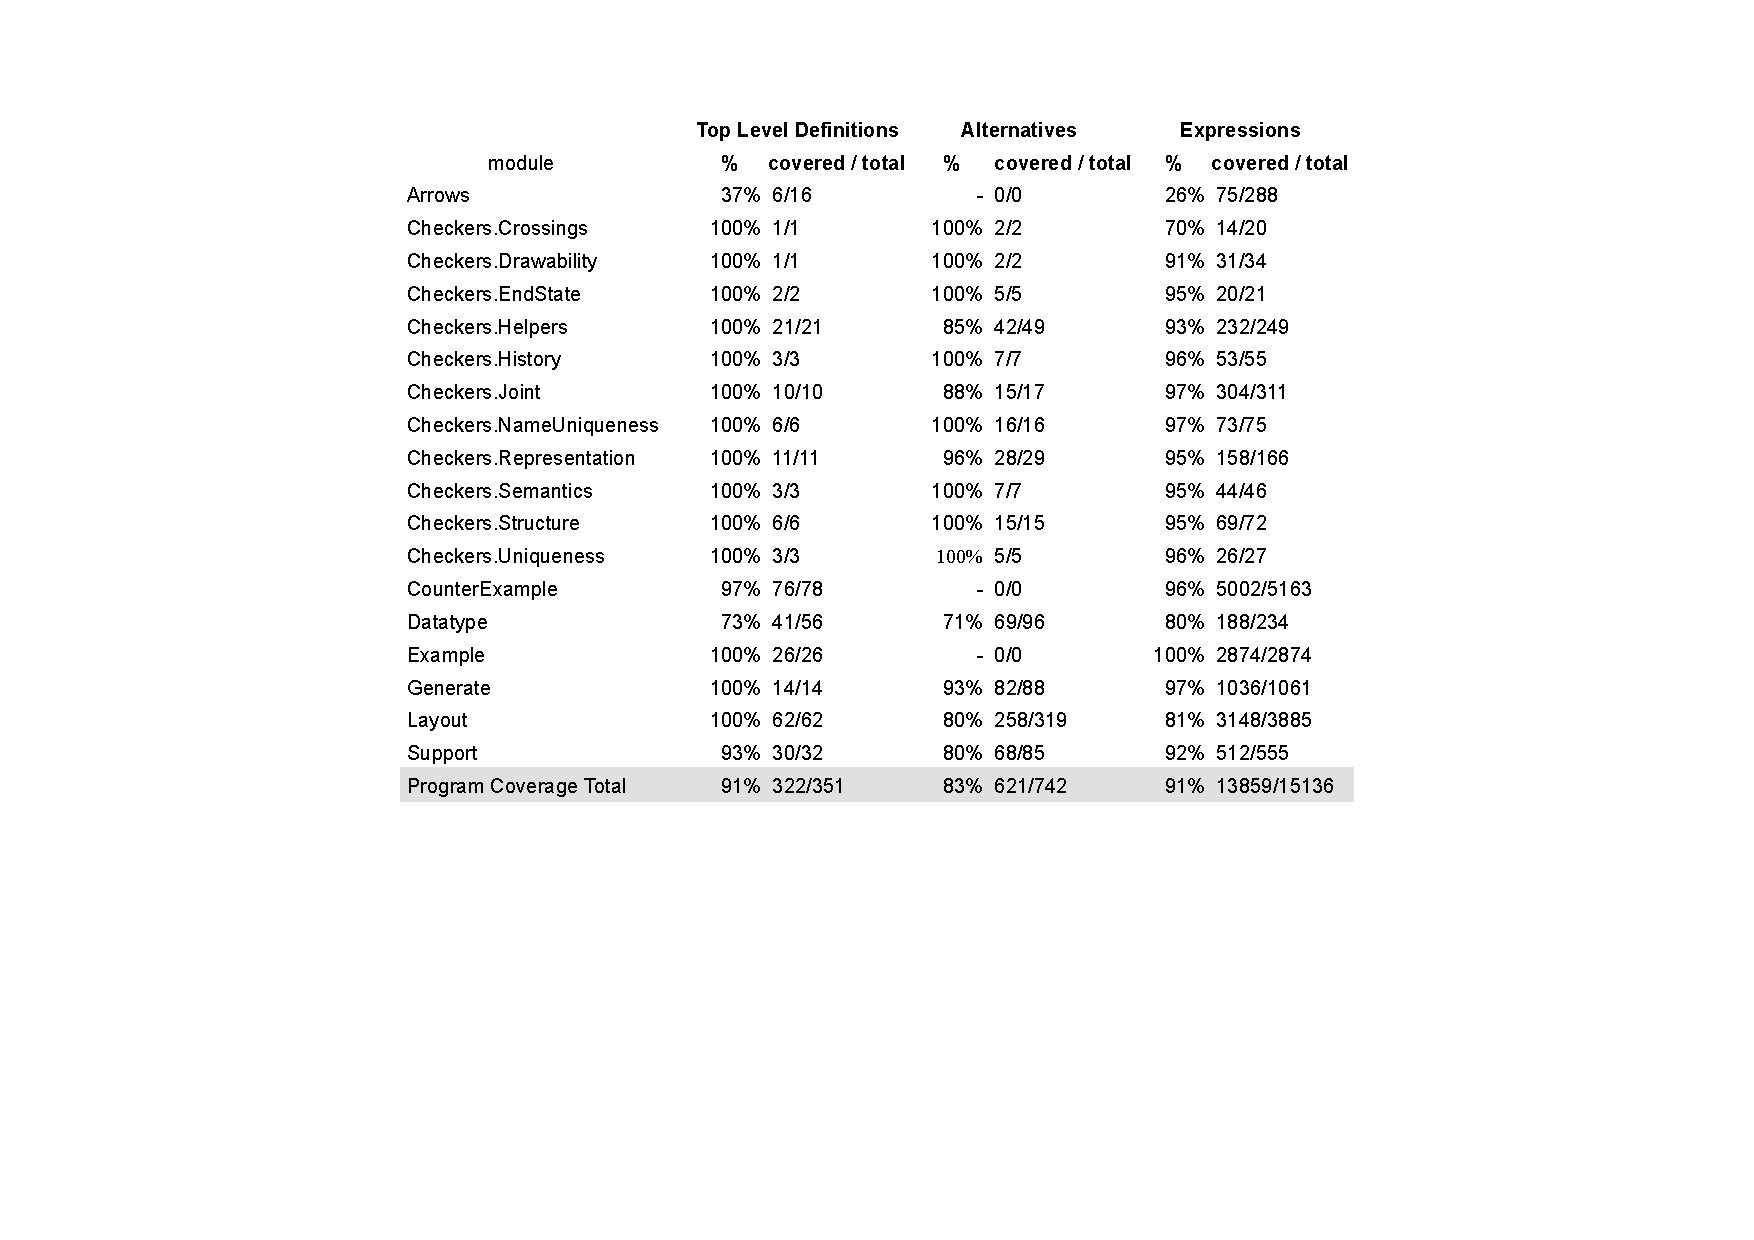
\includegraphics[scale=0.65]{Bilder/coverage1.pdf}
    \caption{coverage output from hpc-markup}
    \label{fig:coverage1}
\end{figure}
\begin{figure}[ht]
    \centering
    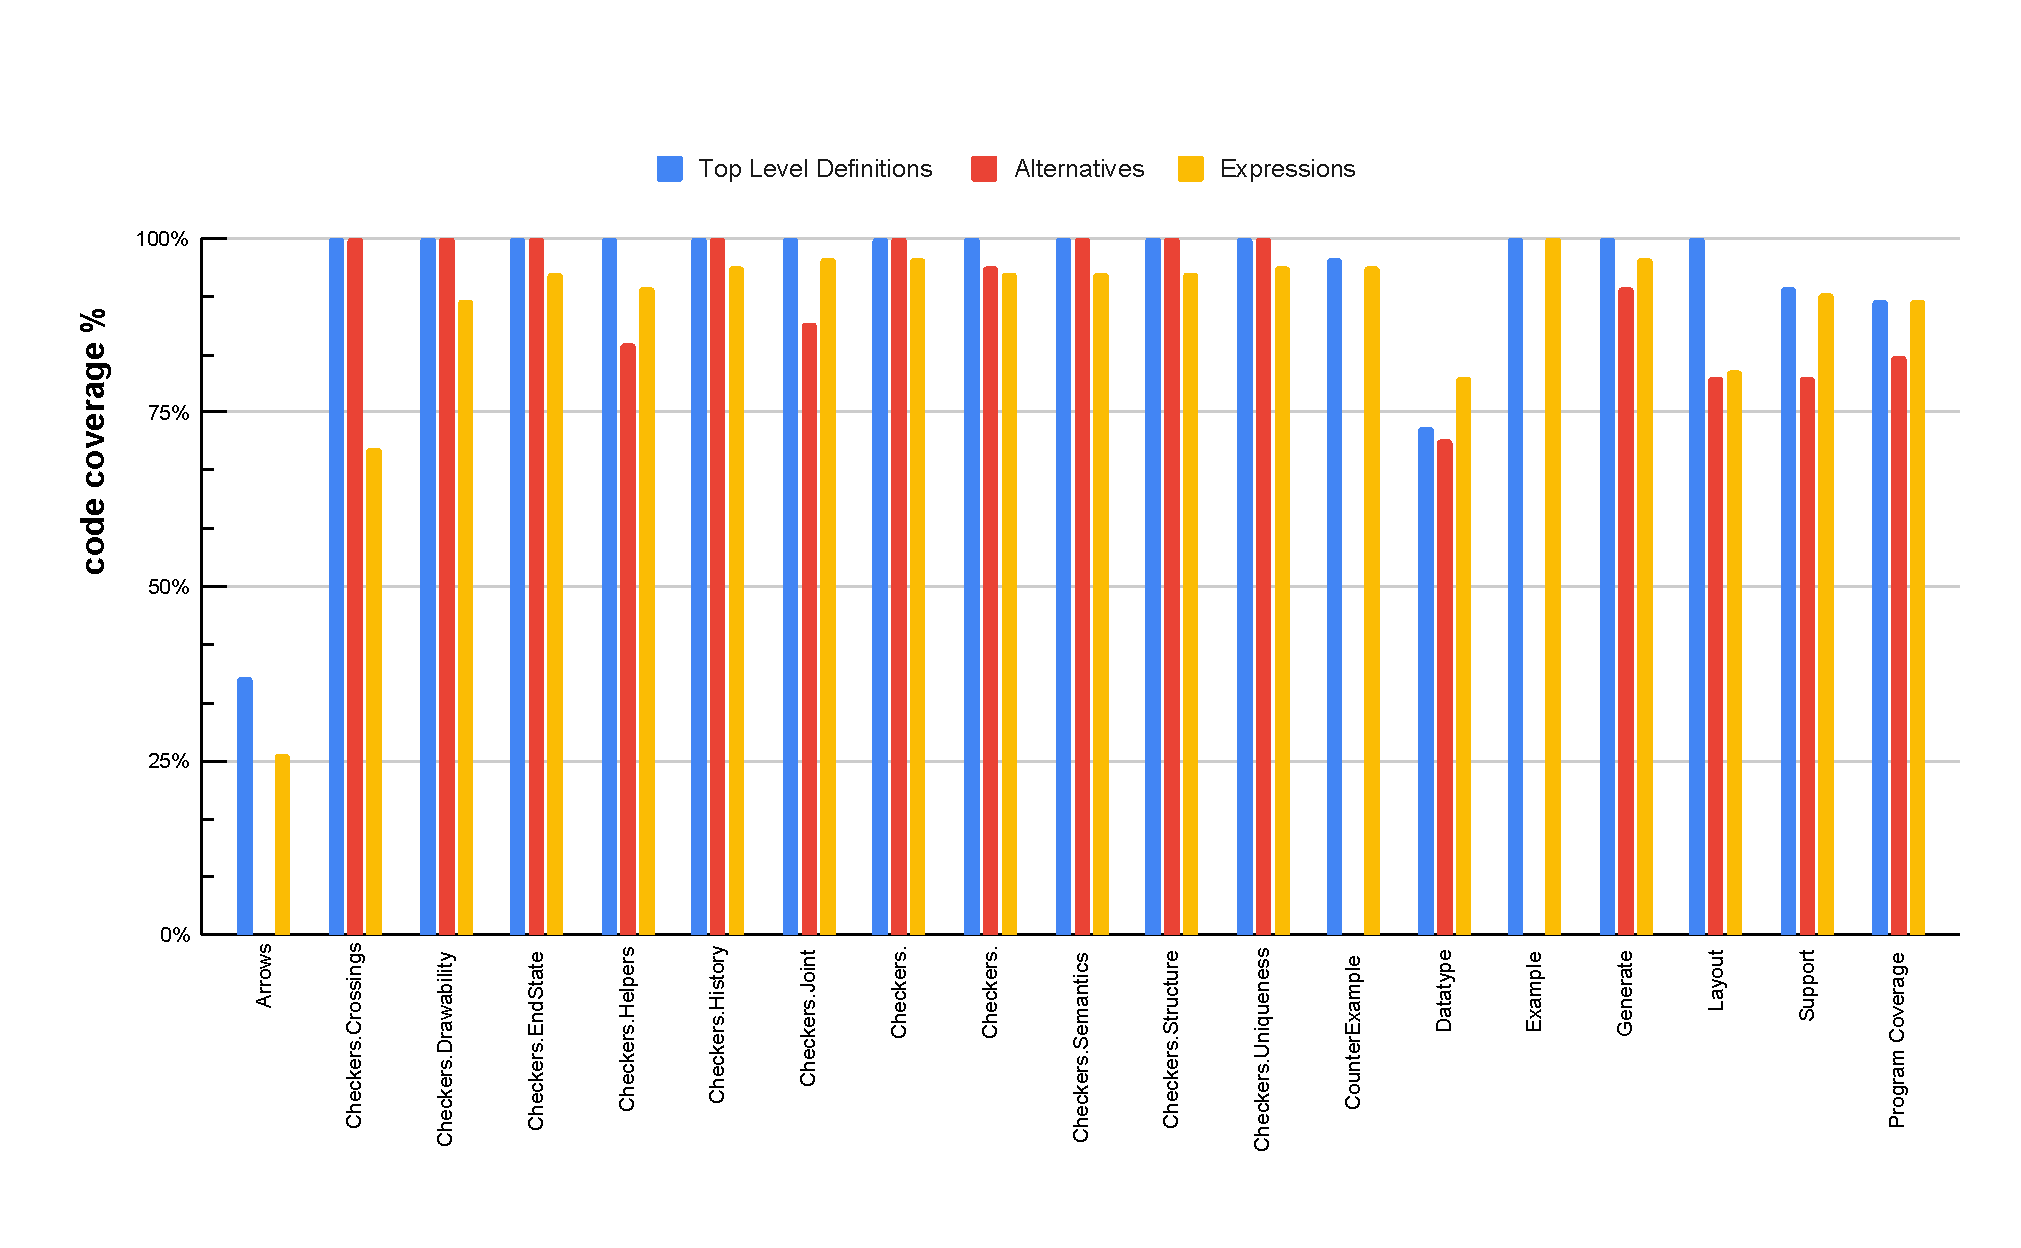
\includegraphics[scale=0.4]{Bilder/coverage2.pdf}
    \caption{coverage}
    \label{fig:coverage2}
\end{figure}
\newpage
\section{Errors Found}
Except for the errors found by fuzzing tests, we encountered another drawing problem by investigating the random generator: discontinuous lines under certain circumstances.At the layer of \verb|StateDiagram C| inside a combine diagram \verb|Connection [2] [4,2,4] "f"| is drawn with a discontinuous line. We might investigate it further in the future.
\begin{figure}[ht]
    \centering
    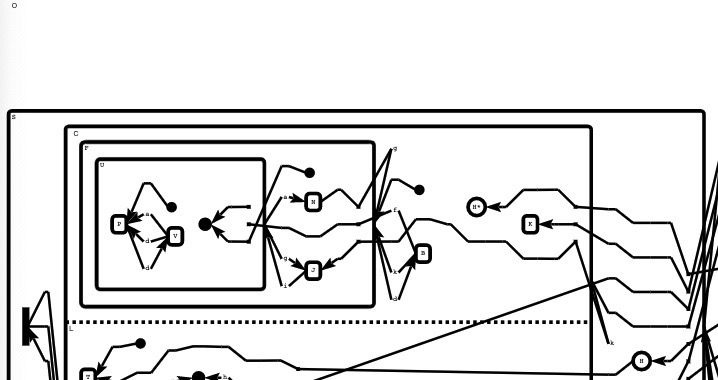
\includegraphics[scale=0.5]{Bilder/error.jpg}
    \caption{discontinuous lines}
    \label{fig:error}
\end{figure}



\chapter{Related and Future Work}
\label{chap:Related and Future Work}

Throughout the paper, we have discussed the automatic generation of non-trivial and conceptual state diagrams to provide exercise tasks in the university lecture setting in the future.

As shown in Figure \ref{fig:sample5},a start state points to a final state.
It does not satisfy the more strict requirement of reachability.
Hence, here are some semantics that may need to realized in the future:
reachability, deadlock, liveness, safety. 
There is an existing model checker \cite{zou/Yiwei2021} for those properties but not in Haskell. 
We also could explore the dynamic semantics \cite{börger_cavarra_riccobene_2000} of UML state machine diagrams.

Moreover, the improvement on the layout strategy, a more controlled branch process for either connection distribution or selection of state types could be further explored. In the Figure \ref{fig:sample6}, the number of connections between different levels and the entry or exit to a composite diagram are not natural. And fixing the drawing errors like self-edges, discontinued lines we mentioned before is essential. We also could give diagram parameters more meaningful names as the process in real software designing. But it is challenging that the transitions between them are limited by the meaning of the diagram.

Except for the state diagram, there is also an automatic generator for the Class/Object diagram \cite{10.1007/978-3-030-35629-3_8,siegburg2020generating} and Petri net formalization in Alloy \cite{ke_wang}. 
Alloy's formalization of the state diagram will also be done in our future work since some constraints are too complex to be realized in Haskell.
Then we compare these two realization ways and find their ad/disadvantages for both approaches.
May combination of the two techniques would give more conceptual and accurate results.
One important thing that needs to be pointed out is in Haskell's formalization that the initial states will never point to something "outside their own level " since the way the Haskell data type works. 
We address a start state from the current state diagram.
Hence this situation should be forbidden in the formalization via Alloy.

\begin{figure}[ht]
    \centering
    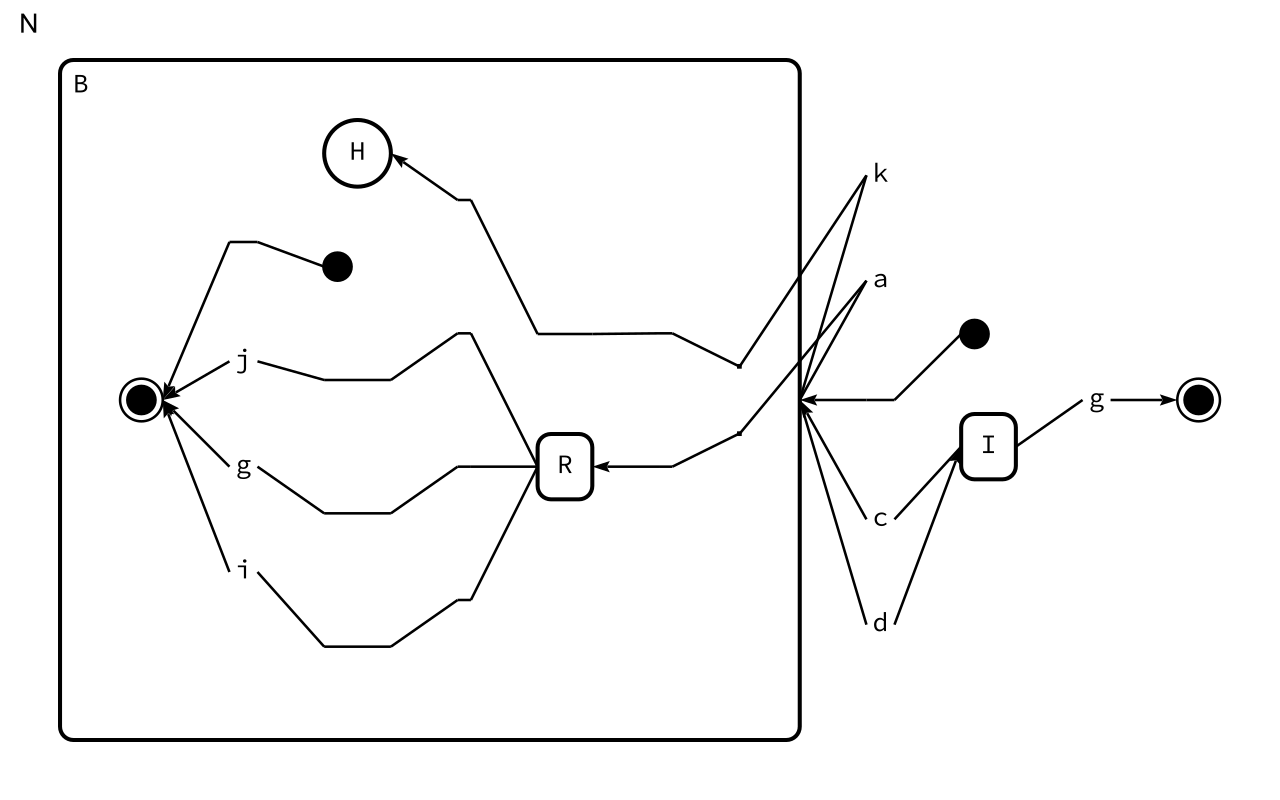
\includegraphics[scale=0.5]{Bilder/sample5.png}
    \caption{sample5}
    \label{fig:sample5}
\end{figure}
\begin{figure}[ht]
    \centering
    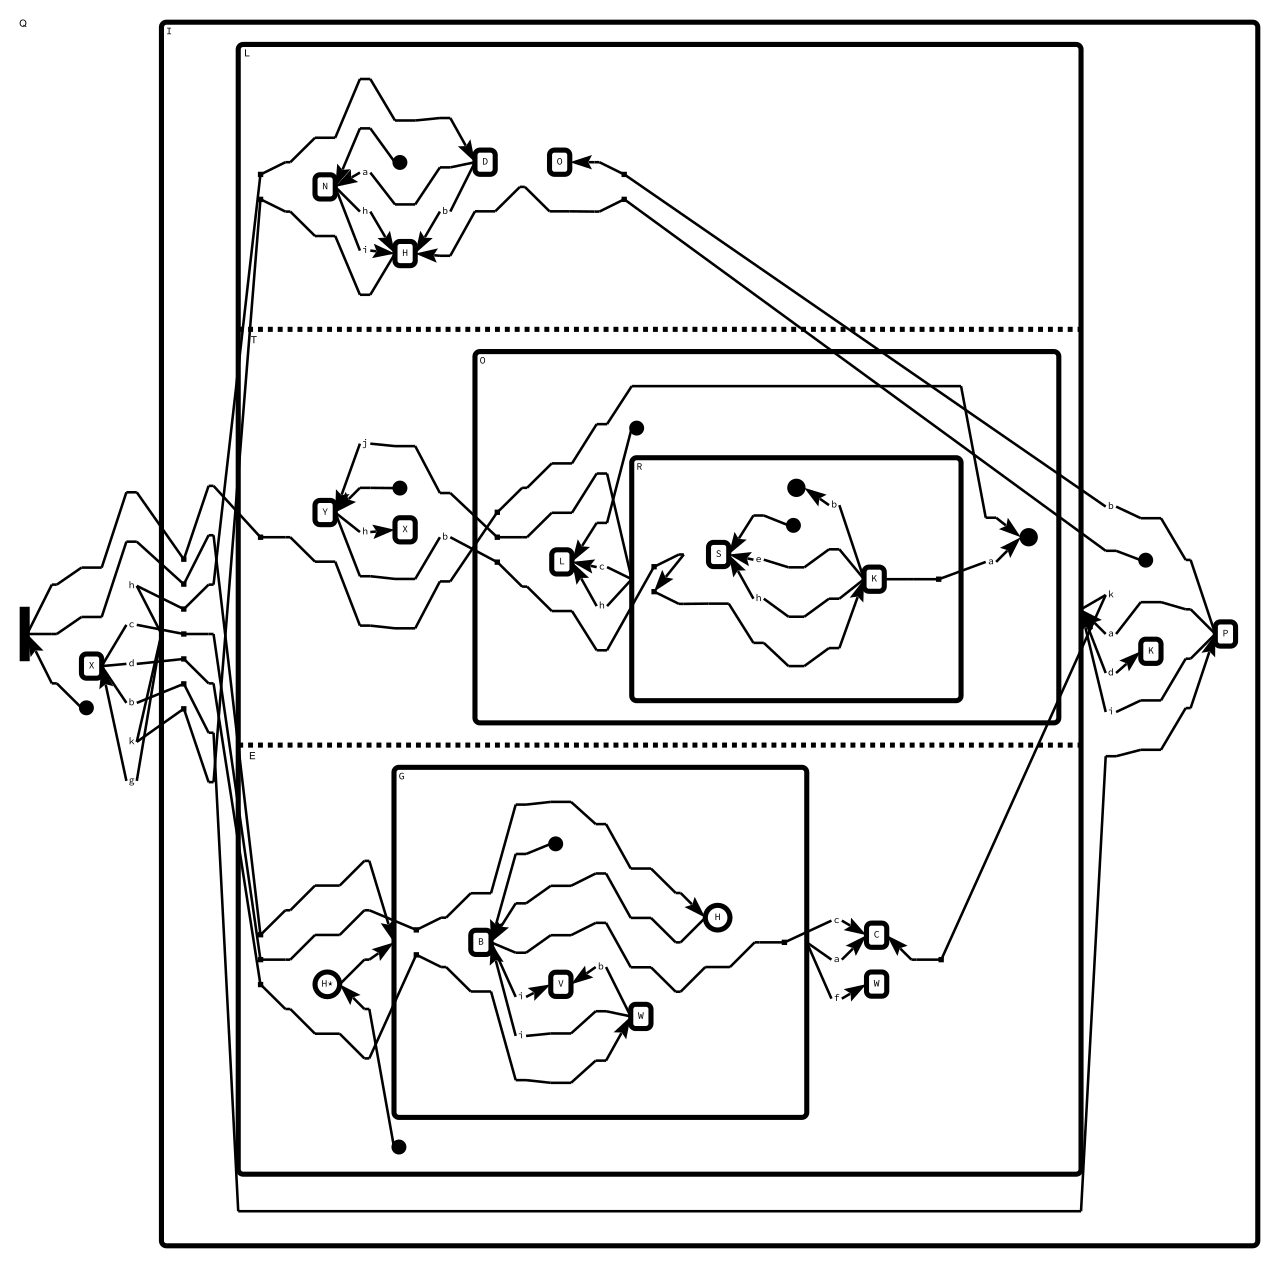
\includegraphics[scale=0.7]{Bilder/sample6.png}
    \caption{sample6}
    \label{fig:sample6}
\end{figure}


% Appendix
\cleardoublepage
\part*{Appendix}
\listoffigures
\printbibliography

% Erklärung
\cleardoublepage
\pagestyle{empty}
\begin{center}
\Large{\textsf{\textbf{Erklärung}}}
\end{center}
\vspace{0.8cm}
Hiermit erkläre ich, dass ich die vorliegende Arbeit ohne fremde Hilfe selbstständig
verfasst und nur die angegebenen Quellen und Hilfsmittel benutzt habe. Ich versichere
weiterhin, dass ich diese Arbeit noch keinem anderen Prüfungsgremium vorgelegt habe.

Duisburg, im Dezember 2021
\\[1cm]
.................................................\\[0.2cm]
Le Zhang 
\pagestyle{empty}
\cleardoubleemptypage

\end{document}
